\noindent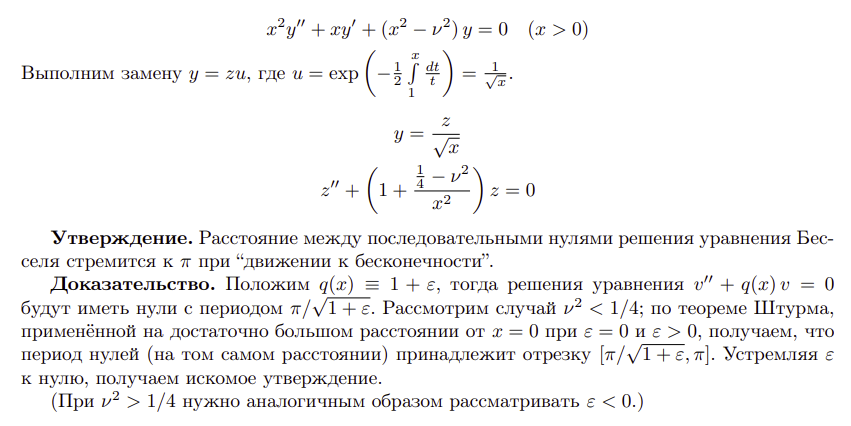
\includegraphics[width=0.95\linewidth]{images/bess.png}

\subsubsection*{Решения}
Доказано, что в общем случае решения уравнения Бесселя не выражаются через композиции коэффициентов уравнения, элементарных функций и их интегралов. Однако эти
решения можно выразить как степенные ряды.

\textbf{Функция Бесселя первого рода}
\begin{equation*}
    J_\nu(x) = \sum\limits_{k=0}^{\infty}{\frac{(-1)^k\Big(\frac{x}{2}\Big)^{2k+\nu}}{\Gamma(k + 1)\Gamma(k+1+\nu)}}
\end{equation*}
где $\Gamma$ -- это гамма-функция: $\Gamma(k+1) = k!$ \;и\; $\Gamma(k+1+\alpha) = (\alpha+1)\ldots(\alpha+k)\Gamma(\alpha+1)$

\subsubsection*{Cвойство решения:}
\begin{center}
    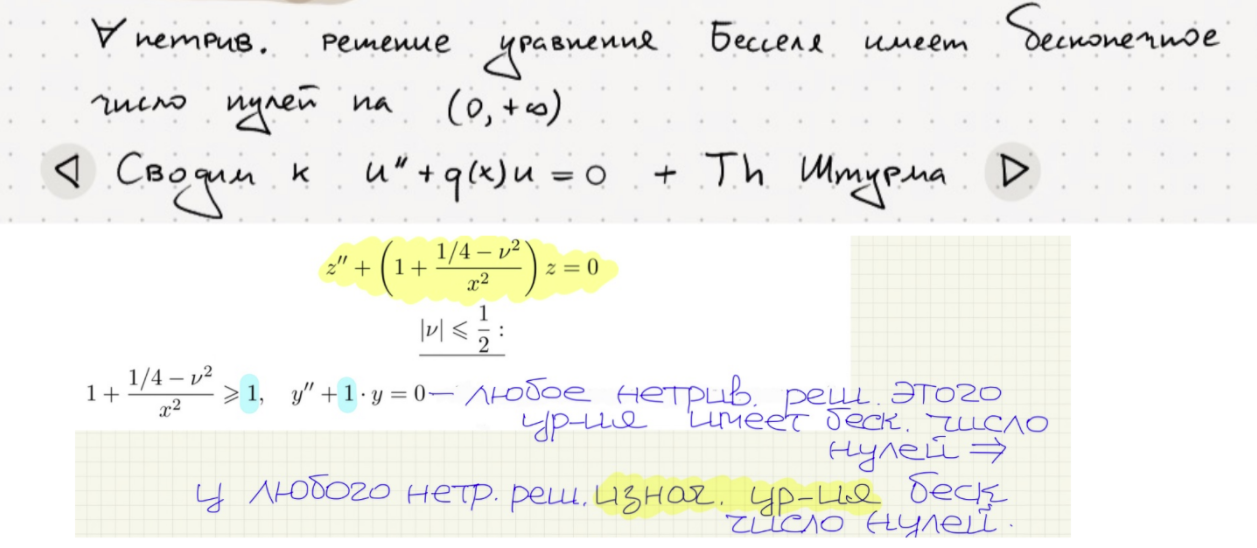
\includegraphics[width=0.95\linewidth]{images/bess_1.png}
\end{center}
\begin{center}
    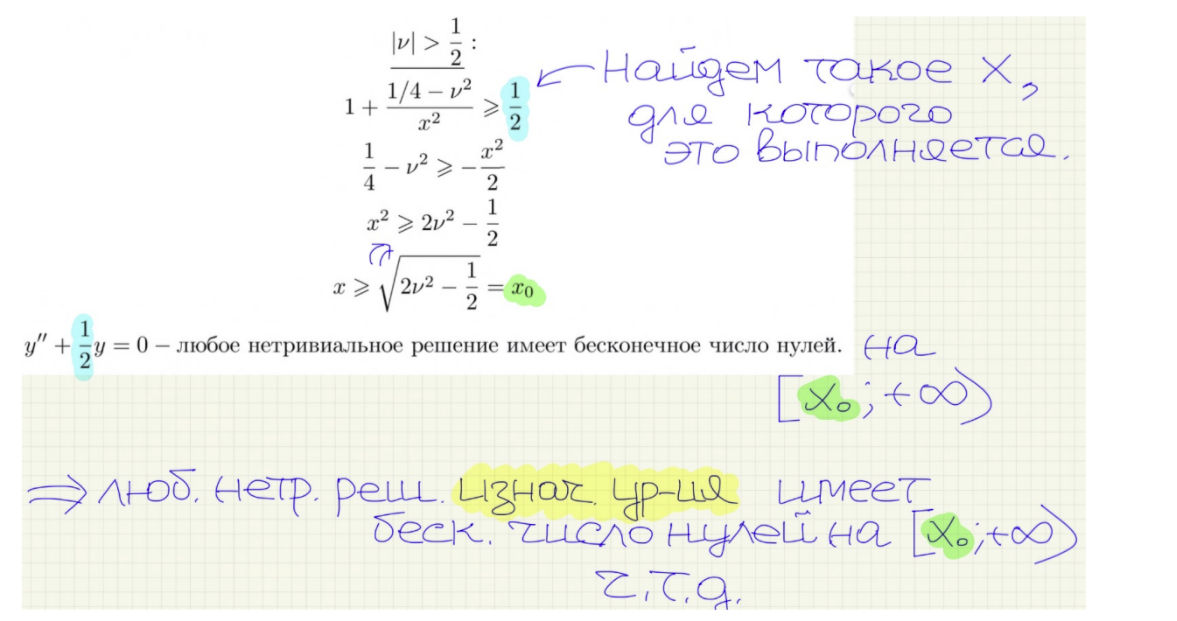
\includegraphics[width=0.95\linewidth]{images/bess_2.png}
\end{center}
\newpage